\section{Proto-MapReduce}
\textbf{The MapReduce implementation used in this prototype is a simplified version} of what discussed in \textit{appendix \ref{the_mapreduce_paradigm}}; said simplifications, while making it \textbf{easier to implement}, have the \textbf{side effect of negatively influencing performances but}, given the available time limitations, they are \textbf{still acceptable in a prototypical context where the focus is to demonstrate the feasibility of mobile devices Contribution}.

\textbf{The first difference comes from how the data are handled}. The MapReduce paradigms handles a number of splits M and applies progressively the Map function to said splits; the intermediate results are grouped by key (using a partitioning function) in order to obtain R (with R<M, typically) partitions which, upon allying the Reduce function, will produce R final results. This \textbf{simplified version}, on the contrary, \textbf{takes the M splits} and, after applying the Map function, \textbf{maintains the original grouping, producing M intermediate results}; said results are then \textbf{computed applying the Reduce function} to each of them, \textbf{producing the M final results}. As a consequence, \textbf{the number of input data regions is equal to the regions in the final results}.

\vspace{10mm}

\begin{figure}[!ht]
    \centering
    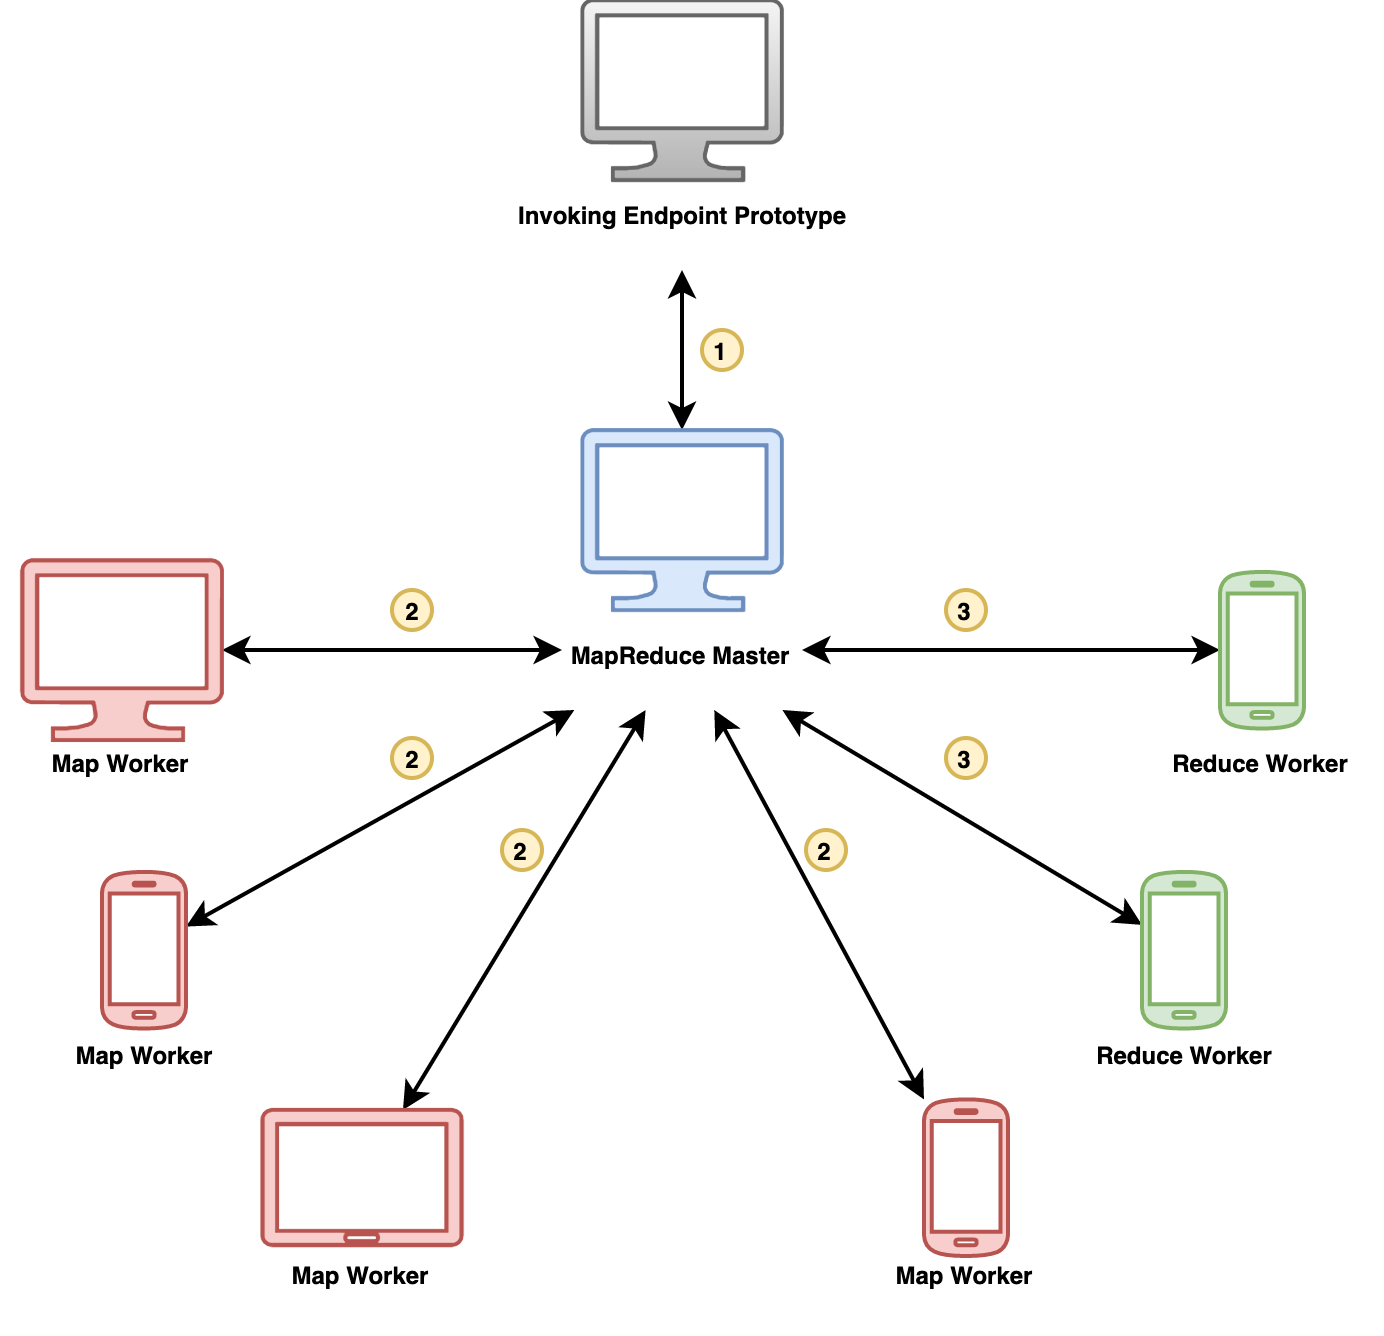
\includegraphics[scale=1]{document/chapters/chapter_6/images/proto_mapreduce.png}
    \caption{Proto-MapReduce Topology}
    \label{fig:proto_mapreduce}
\end{figure}

\textbf{The second important distinction comes from the topology of the connections among the entities involved} in the MapReduce operation. Normally, a Map Worker that has completed a run of the Map function would send, under the coordination of the MapReduce Master, its intermediate results directly to the right Reduce worker; \textbf{in this simplified version a Map Worker that has completed a Map operation sends its results to the MapReduce Master which, after gathering all the Map results for that particular region, will forward the data to an assigned Reduce Worker}. The final topology for the MapReduce Service performed in this prototype is shown in \textit{figure \ref{fig:proto_mapreduce}} and is \textbf{obtained performing these three steps}:
\begin{enumerate}
    \item \textbf{MapReduce Master recruitment}\\
    The Invoking Endpoint Prototype performs a recruitment (seen in \textit{figure \ref{fig:recruitment_messages}}), connecting to a Node which receives a MapReduce Master Job (containing all info about resources requested with the Map and Reduce functions definitions as well). This marks the beginning of the next phase but, in the meantime, the Invoking Endpoint starts sending Tasks to the MapReduce Master (\textit{figure \ref{fig:p2p_messages}}), each containing a data region to compute.
    \item \textbf{Map Workers recruitment}\\
    The MapReduce Master performs a recruitment, requesting the Map Workers specified in its MapReduce Master Job, and it sends a Map Worker Job (containing the Map function) upon every new connection; once all the requested Map Workers are recruited, the next phase can begin, while, at the same time, also starting to send Tasks containing the data to which apply the Map function.
    \item \textbf{Reduce Workers recruitment}\\
    Here the MapReduce Master performs the final recruitment, requesting the Reduce Workers specified in its MapReduce Master Job, sending a Reduce Worker Job (containing the Reduce function) to every new Node recruited. After this recruitment is completed, the MapReduce Master is allowed to send the progressively collected intermediate results to the Reduce Workers. 
\end{enumerate}

\textbf{Once all the data region are computed and the results are collected by the Invoking Endpoint, the P2P connections are closed}, completing the execution.

As can be easily deduced, the Invoking Endpoint Prototype acts as a Master in its P2P connection to the MapReduce Master, while Map and Reduce Workers only act as Slaves in their connection to the same entity, \textbf{making a Node} (the MapReduce Master in this case) \textbf{able to perform both the Master and the Slave roles at the same time}, with the consequence of showing \textbf{that the Map Worker to Reduce Worker connection is perfectly feasible in a future implementation} of these Jobs.

\textbf{Thanks to this topology, every computationally heavy operation is delegated to the Grid's Nodes and, thus, the Invocation can be performed even from a low-spec device}, increasing the versatility of the Grid. 

On a final note, while performing a recruitment, various parameters can be specified about the resources that a device needs to possess; while the Map or Reduce Worker role can be taken by any device, \textbf{the MapReduce Master role is reserved to Desktop devices}. This choice is made \textbf{trying to obtain more stability} for the MapReduce process.  
